\chapter{Neutrino physics}
\label{sec:neutrino}

\epigraph{I have done a terrible thing, I have postulated a particle that cannot be detected.}{Wolfgang Pauli -- "Foreword" by Frederick Reines to "Spaceship Neutrino" by Christine Sutton, (p. xi), 1992. }

%\textit{In chapter 1, I'll remind briefly the SM, its limitations, and give a short introduction to neutrino physics, with a reminder of the present important questions and a state of the art.}


\minitoc

Our understanding of the universe describe it as composed of elementary components called elementary particles, the study of these particles is therefore particles physics. The theoretical model describing these particles and their interactions is the Standard Model (SM), with the exception of the gravitation. It has proven its robustness over the last decades, accounting for most of observed the phenomena with a few exception. This exception are phenomena described as Beyond Standard Model (BSM).

In this chapter in describe briefly the Standard model and its limitations in section \ref{sec:neutrinos:sm}, then delve a bit further in the specificity of neutrinos physics in Section \ref{sec:neutrino:th}.

\section{Introduction to the Standard model}
\label{sec:neutrinos:sm}

The SM categorize the elementary particles into two categories: the \textit{fermions} constituting the matter and the \textit{bosons} that mediate their interaction. The fermions are themselves divided in two categories, the \textit{quark} and the \textit{leptons}. Figure \ref{fig:neutrino:sm} shows the elementary particle and their classification. Each one these particle is characterized by the value of their quantum number the main one being their mass $m$, spin $J$ and electric charge $Q$. The leptons also possess leptonic quantum number $L = 1$ a flavor quantum number $L_{e,\mu,\tau}$ corresponding to their family, electronic, muonic or tauic. The leptons are thus split in three family: the electronic $L_e = 1 \rightarrow (e, \nu_e)$, muonic $L_\mu = 1 \rightarrow (\mu, \nu_\mu)$ and tauic $L_\tau = 1 \rightarrow (\tau, \nu_\tau)$ families, each composed of a charged $Q = 1$ and a neutral particle $Q = 0$. The neutral leptons are named the \textit{neutrinos} represented by the character $\nu$.

\begin{figure}
  \centering
  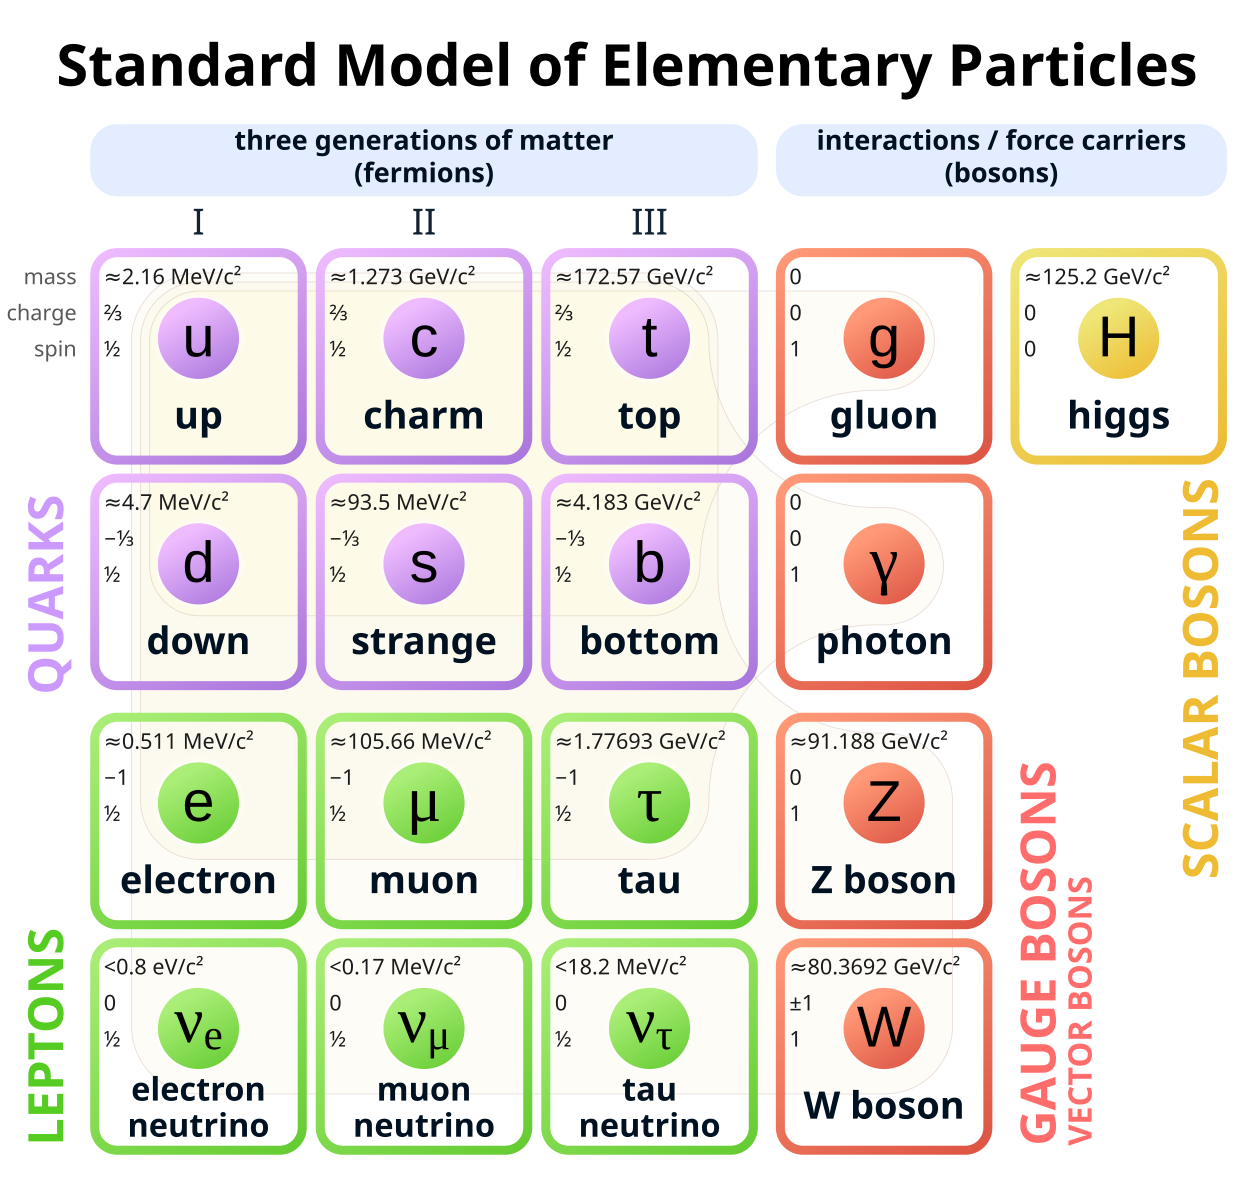
\includegraphics[height=6cm]{images/neutrinos/sm.png}
  \caption{List of the elementary particles in the Standard Model. The antiparticles are not displayed.}
  \label{fig:neutrino:sm}
\end{figure}

Each fermion also possess an antiparticle of opposite electric charge and opposite leptonic and flavour quantum number. Thus the antiparticle of the electron $e (Q=1, L=1, L_e=1)$, the positron is defined $e^+ (Q=-1, L=-1, L_e=-1)$.

The particles of the SM interact with each other via four interactions or forces. Three are described by the SM by the exchange of a boson:
\begin{itemize}
  \item The strong force, described by the exchange of a gluon. Only the quark are sensitive to it. This force is very small range $\sim 10^{-15}$ m, the size of a nucleus. It's the strong force that allow the cohesion of nucleus inside atoms. As its name indicates, it this the strongest of the four interaction.
  \item The electromagnetic force, described by the exchange of a photon. This force has unlimited range, all the charged particles -- quark and charged leptons -- are sensitive to it. It is responsible for every magnetic effect like the bonding of electrons and nucleus. Its relative strength with the strong force is 1/137.
  \item The weak force, carried by the $Z^0$ and $W^{\pm}$ bosons. Every fermions is sensitive to it. Its range is $\sim 10^{-18}$ m, $\sim 0.1\%$ the size of a proton. Its relative strength to the strong force is $10^{-6}$, explaining its name. It is responsible for nuclear beta decay and other similar process. We dinstinguish two types of weak interaction, through neutral -- exchange of a $Z^0$ -- and charged current -- exchange of a $W^{\pm}$ boson.
\end{itemize}

The final force, not described by the standard model, is the gravitational force. It's range is infinite, and concerns every massive ($m \neq 0$) particles. Its relative strength to the strong force is of $6\times 10^{-39}$. Extension to the SM propose a supplementary boson, the graviton, that be the carrier of the gravitational force but it has yet to be detected \cite{ParticleDataGroup:2024cfk, carney_graviton_2024}.

\subsection{Interactions and symmetries}

Symmetries are fundamental components of modern particle physics. As described in Noether's theorem \cite{noether_invariant_1971}, the invariance or non-invariance of the physics law under transformations (translation, rotation, ...), represented by the formal invariance of the SM Lagrangian ${\cal L}$ under those transformation, express the conservation of a quantity.

The invariance of ${\cal L}$ by translation in space characterize the conservation of the momentum, the rotational invariance in space the conservation of the angular momentum, the invariance by translation in time the conservation of energy, etc. If the transformation is continuous, the sum of the quantum numbers is conserved in a interaction.

Invariances under discrete transformation also provide conservation of quantum number. Three discrete transformations are important for the SM:
\begin{itemize}
  \item The parity $P$ symmetry transform $(\vec{x}, t) \rightarrow (-\vec{x}, t)$, reversing the handedness of space. The momentum thus become $\vec{p} \rightarrow -\vec{p}$ and the helicity $\frac{\vec{p} \cdot \vec{s}}{|\vec{p}|}$, where $\vec{s}$ is the spin, change sign.

  \item Reversal of time $T$ where $(\vec{x}, t) \rightarrow (\vec{x}, -t)$, inverting the initial and final state of an interaction $A + B \rightarrow C$ become $C \rightarrow A + B$. The momentum and the spin both change sign, leaving the helicity unchanged.

  \item Charge conjugation $C$, replacing the particles by their antiparticles counterpart and vice-versa, leaving untouched the momentum, spin and helicity.
\end{itemize}

The C, P and their combination CP symmetry was believed to be conserved until 1956, the discovery of their violation \cite{lee_question_1956, wu_experimental_1957, christenson_evidence_1964} in weak interaction revealed the non-triviality of its nature.

The fundamental symmetry CPT, the combination of C, P and T symmetry, is an exact symmetry. It mean that any process where the particles are switched with their anti-particles, spin-projection are of opposite sign and initial and final state are swapped must go with the same probability than the initial process. This implies that the mass, life times, absolute values of electric charge and magnetic moment of particles and antiparticles must be the same.

The strong and electromagnetic interactions are invariants under discrete combined and CP transformations. The weak interaction, is only invariant under CPT.

% Decrire le model standard -> Regarder theses LHC / Olga Kochebina

\subsection{Limits of the standard model}

The SM has been successful at describing a lot of phenomena observed in experiment. However, some questions remains unanswered, among which:

\begin{itemize}
  \item Dark matter and dark energy. Cosmological observation -- the acceleration of the expansion of the universe and the rotational speed of galaxy for example -- indicate the presence of unknown energy and matter in the universe. The $\Lambda$CDM model \cite{bull_beyond_2016, perivolaropoulos_challenges_2022} indicates that only 4.5\% of the total energy in the universe is described by the SM. The supplementary mass -- dark matter -- account for 22.5\% for of the missing energy and the rest is dark energy.
  \item The matter antimatter asymmetry. The universe is mainly made of matter. The deficit of antimatter is allowed, partially, by the CP violation but the magnitude predicted by the SM is not sufficient to explain it quasi-absence.
  \item Fermion masses. The large mass difference between the fermions and is not explained by the SM.
  \item Number of parameters. The SM is composed of 26 numerical parameters that can only be fixed by experimental observations. At least 20 of these parameters are related to flavour physics. In electroweak theory nothing dictates the values of the interaction couplings and masses.
  \item Strong CP problem. Theoretically it is possible to have violation of CP symmetry in the strong interaction sector also. Experimentally, however, no such asymmetry has been found, implying that the coefficient of this term is very close to zero. This fine tuning is also considered unnatural.
  \item Non-unification of couplings. The gauge couplings of the SU(3), SU(2) and U(1) groups are independent quantities. Due to higher-order corrections, each of these is actually a function of the typical energy scale Q relevant to the process. In many grand unified theories the three gauge couplings are predicted to meet at some high energy unification. However, this unification does not occur when the couplings extrapolated using the SM model expression.
  \item Gravitation. The SM do not include the Gravitational interactions and is incompatible with the general relativity.
\end{itemize}


% \marginpar{Limite du model standard - Interessant/justifier etudier les neutrinos -> violation de CP ? Pb des masses ?}
\section{The Neutrinos}
\label{sec:neutrino:th}

As introduced in the precedent section, the neutrino are the neutral leptons of the Standard Model (SM). It has been first theorized by Wolfgang Ernst Pauli in 1978 \cite{pauli_dear_1978} to solve the problem of the $\beta$-decay continuous spectrum. Indeed if the $\beta$-decay was a two body reaction $^A_Z X \rightarrow ^A_{Z + 1}Y + e^{-}$, the conservation of momentum would force the charged lepton to be mono-energetic, but the measured spectrum was continuous. To solve this problem Pauli theorise the emission of a neutral particle $^A_Z X \rightarrow ^A_{Z + 1}Y + e^{\pm} + \nu$, the neutrino. This particle has to be light, neutral and interact weakly with matter.

We must wait 1956 for a collaboration lead by Frederick Reines and Clyde Cowan for the first observation of the neutrino \cite{reines_neutrino_1956, cowan_detection_1956} via the Inverse Beta Decay (IBD) reaction
\begin{equation}
  \bar{\nu} + p \rightarrow e^+ + n
\end{equation}

Following this discovery, numerous experiment were setup to study it properties. Some of the notable discovery include the discovery in 1962, by a collaboration lead by Leon Lederman, Melvin Schwartz and Jack Steinberg, of the neutrino muonic flavor \cite{danby_observation_1962}.

Soon after, the Homestake experiment, which was measuring the neutrino produced by the proton-proton fusion cycle in the sun, report a deficit of factor $\sim 3$ \cite{davis_review_1994} in comparison to the Standard Solar Model predictions. This anomaly, referred as the \textit{solar neutrino problems} remained unexplained until the neutrino oscillation was theorized and proven. Bruno Pontecorvo first suggest a $\nu \leftrightarrow \bar{nu}$ oscillation \cite{pontecorvo_mesonium_1957}, later revisited by Maki et al. to a two flavor oscillation $\nu_e \leftrightarrow \nu_\mu$ \cite{maki_remarks_1962}. The discovery of the $\tau$ lepton 1976 \cite{perl_evidence_1975} and it associated neutrino $\nu_\tau$ \cite{kodama_observation_2001} lead to the extension to three flavor oscillation.

This three flavor oscillation was confirmed by the observation of the $\nu_\mu \leftrightarrow \nu_\tau$ oscillation \cite{fukuda_evidence_1998}.

\subsection{Coupling and interactions}

The SM, as originally defined, contains no right-handed neutrino (right helicity) neutrino since only left-handed neutrino have been observed \cite{goldhaber_helicity_1958}, inducing that the neutrino are massless. Neutrino actually do have a very small mass $m_\nu < 0.45eV$ at 90\% confidence level \cite{aker_direct_2024}. They only couple -- interact -- through the $W^{\pm}$ and $Z^0$ bosons. The coupling with a $W^{\pm}$ boson is the \textit{charged current}, a charge is exchanged via the $W$ boson and coupling with $Z^0$ is the neutral current, no charge is exchanged. The feynman diagrams representing those interaction are presnted in figure \ref{fig:neutrinos:currents}.

\begin{figure}
  \centering
  \begin{subfigure}[t]{0.48\linewidth}
    \centering
    \feynmandiagram[horizontal=a to b] {
      a -- [boson, edge label=\(W^{\pm}\)] b,
      f1 [particle=\(\nu_l\)] -- [fermion] b -- [fermion] f2 [particle=\(l\)]
    };
  \end{subfigure}
  \hfill
  \begin{subfigure}[t]{0.48\linewidth}
    \centering
    \feynmandiagram[horizontal=a to b] {
      a -- [boson, edge label=\(Z^0\)] b,
      f1 [particle=\(\nu\)] -- [fermion] b -- [fermion] f2 [particle=\(\nu\)]
    };
  \end{subfigure}
  \caption{Feynman diagrams of the charged current (\textbf{on the left}) and the neutral current (\textbf{on the right}) for a lepton $l$ and it corresponding neutrino $\nu_l$.}
  \label{fig:neutrinos:currents}
\end{figure}

As explained in Section \ref{sec:neutrinos:sm}, those interactions preserve the leptonic quantum number $L$. In the absence of neutrino mass, the leptonic flavour numbers $L_e$, $L_\mu$ and $L_\tau$ are also exactly conserved. However, the existence of neutrino masses allow for lepton flavour violating transition such as the oscillation $\nu_\alpha \rightarrow \nu_{\beta \neq \alpha}$ but also process such as $\mu^+ \rightarrow e^+ + \gamma$ or $\mu^+ \rightarrow e^+ e^+ e^-$, the later that are heavely suppressed -- their probability to happens is extremely low in comparison to other process -- in abscence of new physics \cite{glashow_weak_1970}.


%\subsubsection{First theories}

%\subsubsection{Discovery}

%\subsubsection{Milestones and anomalies}

\subsection{Oscillation}
\label{sec:th:osc}

The masses of neutrinos allow them to oscillate between flavor states, more striclty speaking, their mass induce a mismatch between the \textit{flavour states} $\ket{\nu_e}$, $\ket{\nu_\mu}$ and $\ket{\nu_\tau}$ which are the state in which the particle interact -- the states in the diagrams in Figure \ref{fig:neutrinos:currents} -- and the \textit{mass states} $\ket{\nu_1}$, $\ket{\nu_2}$ and $\ket{\nu_3}$ which hold the momentum and mass of the particle.

Thus the flavour state $\ket{\nu_\alpha}$ can be written
\begin{equation}
  \ket{\nu_\alpha} = \sum_{i=1}^3 U_{\alpha, i} \ket{\nu_i}
\end{equation}
and reciprocely
\begin{equation}
  \ket{\nu_i} = \sum_{\alpha \in e,\mu,\tau} U^*_{\alpha, i} \ket{\nu_\alpha}
\end{equation}
where $i$ indexes the masse states, $\alpha$ the flavour states and $U_{\alpha, i}$ are mixing coefficients. In the three families framework, this mixing is represented by the $3 \times 3$ Pontecorvo-Maki-Nakagawa-Sakata matrix \cite{maki_remarks_1962} $U_{\text{PMNS}}$
\begin{equation}
  \begin{pmatrix}
    \ket{\nu_e} \\
    \ket{\nu_\mu} \\
    \ket{\nu_\tau}
  \end{pmatrix} = U_{\text{PMNS}} \begin{pmatrix}
    \ket{\nu_1} \\
    \ket{\nu_2} \\
    \ket{\nu_3}
  \end{pmatrix} = \begin{pmatrix}
  U_{e1} & U_{e2} & U_{e3} \\
  U_{\mu 1} & U_{\mu 2} & U_{\mu 3} \\
  U_{\tau 1} & U_{\tau 2} & U_{\tau 3}
  \end{pmatrix} \begin{pmatrix}
    \ket{\nu_1} \\
    \ket{\nu_2} \\
    \ket{\nu_3}
  \end{pmatrix}
\end{equation}
This matrix is considered to be unitary but this property still need to be corroborated \cite{parke_unitarity_2016}. Now, considering a neutrino produces as $\ket{\nu_\alpha}$ that propagate over a distance $x$ during a time $t$, the Schrödinger equation \cite{schrodinger_undulatory_1926} can be written as:
\begin{equation}
  \label{eq:neutrino:schro}
  \ket{\nu_\alpha(x, t)} = \sum_{i=1^3} U_{\alpha, i} e^{-i(E_it-p_ix)} \ket{\nu_i}
\end{equation}
where $E_i$ an $p_i$ stand for the energy and momentum of the neutrino mass states respectively. By going back from the mass space to the flavour space, Eq. \ref{eq:neutrino:schro} become:
\begin{equation}
  \ket{\nu_\alpha(x, t)} = \sum_{\beta \in e,\mu,\tau} U^*_{\beta, i} \left( \sum_{i=1^3} U_{\alpha, i} e^{-i(E_it-p_ix)} \right) \ket{\nu_\beta}
\end{equation}

A neutrino created as $\nu_\alpha$ thus propagate as the linear superposition of the three flavor states. Because the mass of the neutrino is extremely, we can consider that they are ultra-relativistic ($E \sim p >> m$). Using natural units $(c = \bar{h} = 1)$:
\begin{equation}
  \label{eq:neutrino:e_eq_p}
  E_i = \sqrt{p^2 + m_i^2} \simeq p + \frac{m_i^2}{2p} \simeq E + \frac{m_i^2}{2E}
\end{equation}
then the probability to observe a neutrino produced in state $\ket{\nu_\alpha}$ in a state $\ket{\nu_\beta}$ can be written \footnote{Actually Eq. \ref{eq:neutrino:e_eq_p} and \ref{eq:neutrino:prob} make a few more assumptions, such as the fact that every mass state have the same momentum, ``Paradoxes of Neutrino Oscillations'' from Akhmedov and Smirnov \cite{akhmedov_paradoxes_2009} go through them and demonstrate the validity of the method presented in this chapter.}:
\begin{equation}
  \label{eq:neutrino:prob}
  P_{\nu_\alpha \rightarrow \nu_\beta} = | \braket{\nu_\beta}{\nu_\alpha} |^2 = \sum_{i,j=1}^3 U^*_{\alpha,i} U_{\beta,i} U^*_{\alpha, j} U_{\beta, j} e^{-i \frac{\Delta m^2_{ji} L}{2E}}
\end{equation}
where $L = ct$ is the propagation distance of the neutrino, $E$ is the neutrino energy and $\Delta m^2_{ji} = m^2_j - m^2_i$ is the \textit{mass splitting}, the difference between the square of the eigenvalues of two mass states.

The PMNS matrix can also also be decomposed in three rotational matrices:
\begin{equation}
  U_{\text{PMNS}} = \begin{pmatrix}
    1 & 0 & 0 \\
    1 & \cos \theta_{23} & \sin \theta_{23} \\
    1 & -\sin \theta_{23} & \cos \theta_{23} \\
  \end{pmatrix} \begin{pmatrix}
    \cos \theta_{13} & 0 & \sin \theta_{13} e^{-i\delta}\\
    0 & 1 & 0 \\
    -\sin \theta_{13} e^{-i\delta} & 0 &  \cos \theta_{13} \\
  \end{pmatrix} \begin{pmatrix}
    \cos \theta_{12} & \sin \theta_{12} & 0 \\
    -\sin \theta_{12} & \cos \theta_{12} & 0 \\
    0 & 0 & 1 \\
  \end{pmatrix}
\end{equation}
where the parameters $\theta_{12}$, $\theta_{23}$, $\theta_{13}$ are the \textit{mixing angles}. The parameter $\delta$ is a CP violation phase that quantify the matte-antimatter asymmetry in the leptonic sector. The parameters $\theta_{12}$ and $\Delta m^2_{21}$ are commonly attributed to a so-called \textit{solar sector} while the parameters $\theta_{13}$ and $\Delta m^2_{31}$ belong to the \textit{reactor sector} and $\theta_{23}$ and $\Delta m^2_{32}$ the \textit{atmospheric sector}. The neutrino oscillation is this characterized by 7 parameters: the three mixing angles $(\theta_{12}, \theta_{13}, \theta_{23})$, the three mass splitting $(\Delta m^2_{21}, \Delta m^2_{31}, \Delta m^2_{32})$ and the CP violation phase $\delta$.

The neutrinos interact weakly with matter. But even so, the travel through dense matter, such as earth crust, can impact their propagation probability. These \textit{matter effects} where introduced for the first time by Lincoln Wolfenstein, Stanislas Mikheyev and Alexei Smirnov in 1978 \cite{wolfenstein_neutrino_1978}. They result from forward elastics scattering of neutrinos with the medium (the momentum of the neutrino is unchanged). The charge and neutral current feynman diagrams are presented in Figure \ref{fig:neutrinos:msw}. This result in a supplementary potential in the Hamiltonian, impacting the oscillation probability. For earth crust density, matter effect must be consider the neutrino travel several hundreds of kilometers in it.


\begin{figure}[ht]
  \centering
  \begin{subfigure}[t]{0.48\linewidth}
    \centering
    \feynmandiagram[vertical=a to b] {
      f1 [particle=\(\nu_e\)] -- [fermion] a -- [fermion] o1 [particle=\(e^{-}\)],
      a -- [boson, edge label=\(W^{-}\)] b,
      f2 [particle=\(\nu_e\)] -- [anti fermion] b -- [anti fermion] o2 [particle=\(e^{-}\)]
    };
  \end{subfigure}
  \begin{subfigure}[t]{0.48\linewidth}
    \centering
    \feynmandiagram[vertical=a to b] {
      f1 [particle=\(\nu_{e, \mu, \tau}\)] -- [fermion] a -- [fermion] o1 [particle=\(\nu_{e, \mu, \tau}\)],
      a -- [boson, edge label=\(Z^{0}\)] b,
      f2 [particle={$e^{-},p,n$}] -- [anti fermion] b -- [anti fermion] o2 [particle={$e^{-},p,n$}]
    };
  \end{subfigure}
  \caption{Feynman diagrams of the of charged current matter effect (\textbf{on the left}) and the neutral current matter effect (\textbf{on the right}). Only the electronic neutrino is sensitive to charged current, whereas every neutrinos are sensitive to neutral current.}
  \label{fig:neutrinos:msw}
\end{figure}

\subsection{Phenomenology}

The neutrinos experiments can be divided in two main categories: the disappearance experiments, which observe a deficit of a specific flavour of neutrinos in the detector in comparison with the expected source flux, and the appearance experiments that search for an excess of a flavour. By placing them at different distances -- baselines -- we can favor the appearance or disappearance of different neutrino flavor. As an illustration of the effect of the baseline, the survival probability of $\bnue$ with respect of the baseline is presented in Figure \ref{fig:neutrino:baseline_effect}.

\begin{figure}[ht]
  \centering
  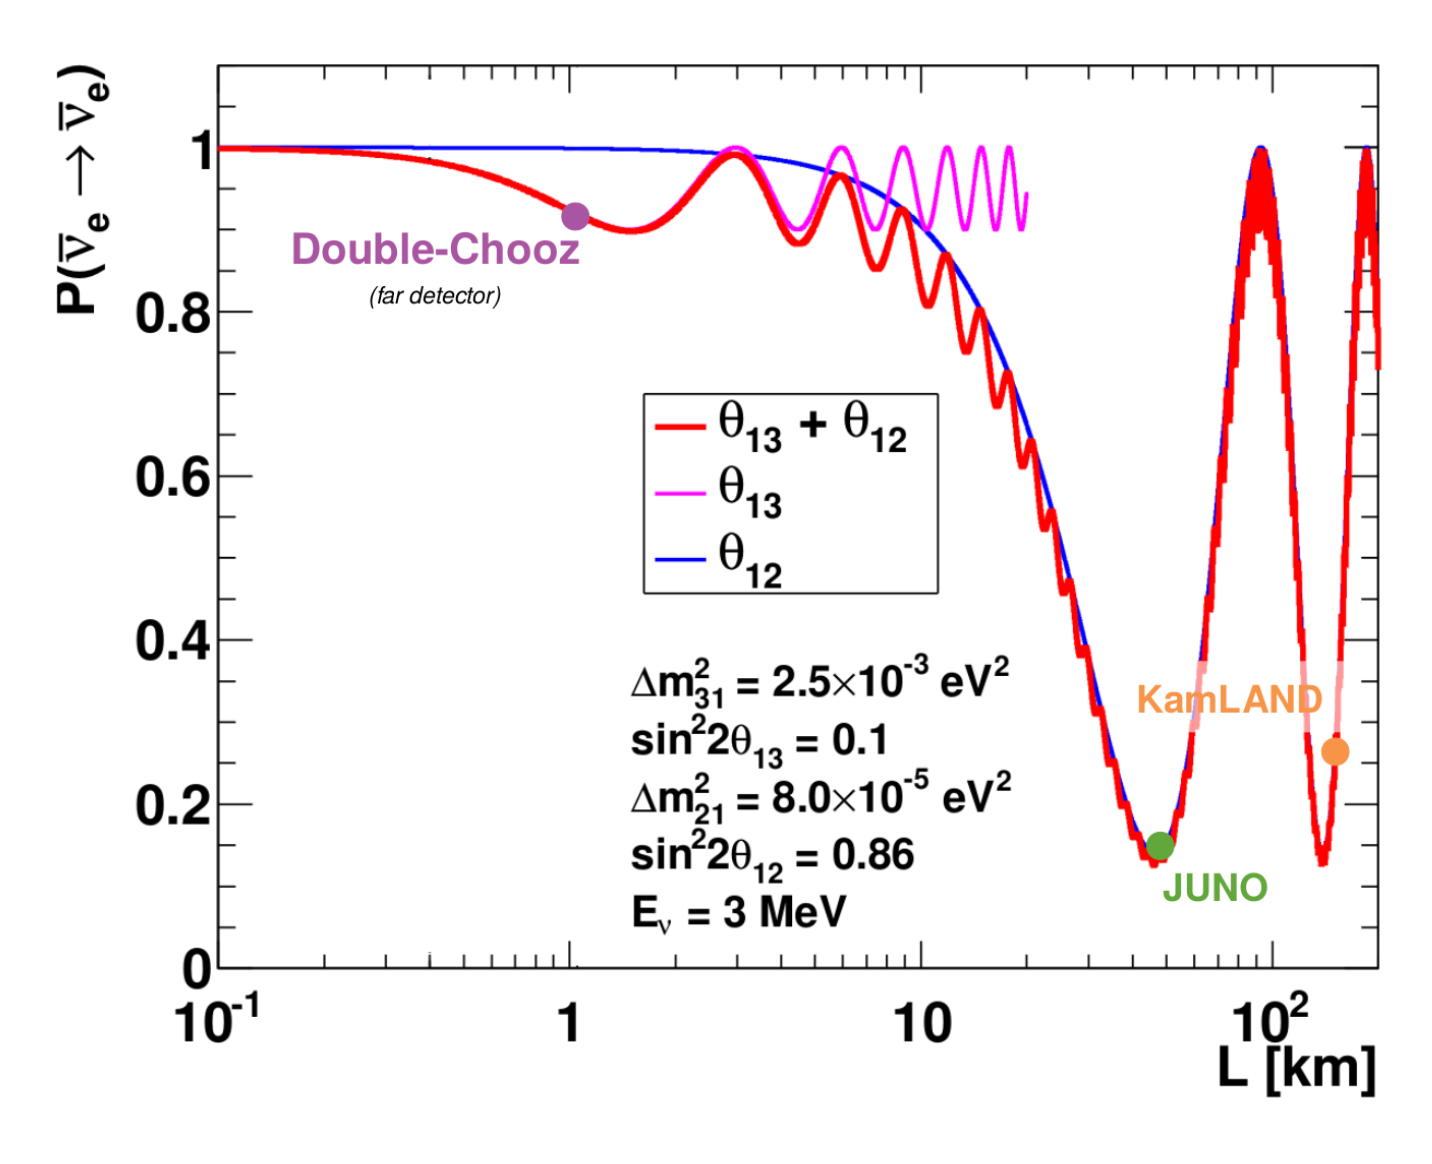
\includegraphics[height=7cm]{images/neutrinos/baseline_effect.png}
  \caption{Survival probability of $\bar{\nu}_e$ as a function of the baseline. The energy of the neutrinos is 3 MeV. The baseline of Double-Chooz, JUNO and KamLAND are reported. Figure taken from Ref. \cite{lebrin_towards_2022}.}
  \label{fig:neutrino:baseline_effect}
\end{figure}

\subsubsection{Solar sector ($\theta_{12}$, $\Delta m^2_{21}$)}

The measurement of the solar sector parameters $\theta_{12}$ and $\Delta m^2_{21}$ has been done in two different way. From the measurements of the solar neutrino flux in experiments like Super Kamiokande \cite{super-kamiokande_collaboration_solar_2016} and by extracting the parameter from the reactor $\bnue$ spectrum, as done by the KamLand-Zen experiment \cite{suzuki_results_2005, kamland_collaboration_reactor_2013}. Those results are further constrained by measurements of short-baseline experiment and accelerator data. The Particle Data Group in its latest edition \cite{ParticleDataGroup:2024cfk} report the following value
\begin{equation*}
  \sin^2\theta_{12} = 0.307^{+0.013}_{-0.012}
\end{equation*}
\begin{equation*}
  \Delta m^2_{21} = 7.53 \pm 0.18 \cdot 10^{-5} \text{ eV}^2
\end{equation*}
The intervals are 68\% confidence level. The invariance CPT is assumed.

\subsubsection{Reactor sector ($\theta_{13}$)}


\subsection{Open questions}
